\documentclass[a4paper]{article}
%\usepackage{fixltx2e} % LaTeX patches, \textsubscript
%\usepackage{cmap} % fix search and cut-and-paste in Acrobat
\usepackage[T1]{fontenc}
\usepackage[utf8]{inputenc}
\usepackage{amsmath}
\usepackage{graphicx}
\usepackage{mathptmx} % Times
\usepackage[scaled=.90]{helvet}
\usepackage{courier}
\usepackage[margin=0.5in]{geometry}
\usepackage{xcolor}
\usepackage{longtable}
%%% User specified packages and stylesheets
\DeclareGraphicsExtensions{ %
    .pdf,.PDF,%
    .png,.PNG,%
    .jpg,.mps,.jpeg,.jbig2,.jb2,.JPG,.JPEG,.JBIG2,.JB2}
\title{PyRETIS --- RETIS analysis}
\author{}
\date{}

\begin{document}
\maketitle
\noindent PPRETIS analysis report generated by PyRETIS version 3.0.3
on 19.04.2026 12:15:24.
\\
\noindent The main results are:
\begin{itemize}
\item The crossing probability:
$P_{\text{cross}} =$ \colorbox{blue!30}{ $nan$ }  $\pm$ $nan$ $\%$

\item The upper estimate of the initial flux (unit: 1/time-unit):
$f_A =$ \colorbox{blue!30}{ $5.384615385 \times 10^{2}$ }  $\pm$ $38.518963075$ $\%$

\item The rate constant (unit: 1/time-unit):
$k_{AB} = $ \colorbox{blue!30}{ $nan$ }  $\pm$ $nan$ $\%$



\item Matching factor between the two [0] ensembles:
$\xi =$ \colorbox{blue!30}{ $1.000000000$ } $\pm$  $0.000000000 \times 10^{0}$ $\%$

\item The time spent in the reference bin (unit: time-unit/
	OP-unit):
$\frac{\tau_{{\mathrm{ref}},[{0^-}{'}]}}{dz} =$ \colorbox{blue!30}{ $0.000000000 \times 10^{0}$ }
$\pm$ $nan$  $\%$

\item The permeability (unit: OP-unit/ time-unit):
$P =$ \colorbox{blue!30}{ $nan$ } $\pm$ $nan$  $\%$



\end{itemize}
\noindent Detailed results are given below for the different path
ensembles and the overall results are summarized
in the last section.

\begin{center}



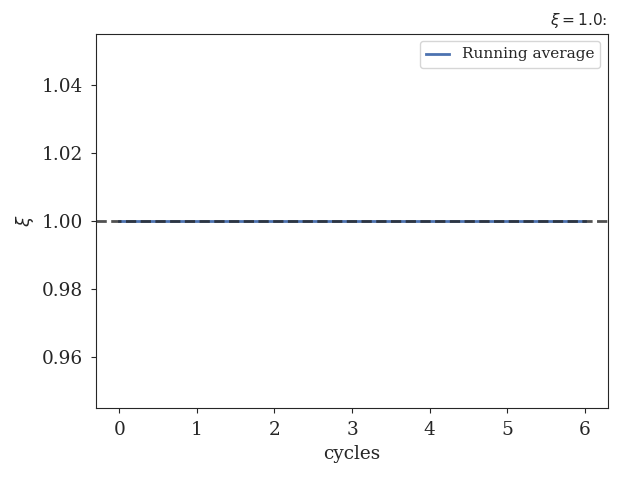
\includegraphics[width=0.33\linewidth]{xirun.png}
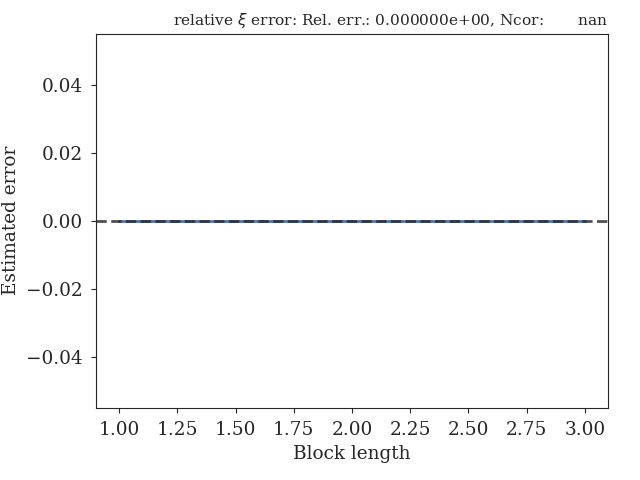
\includegraphics[width=0.33\linewidth]{xierr.png}
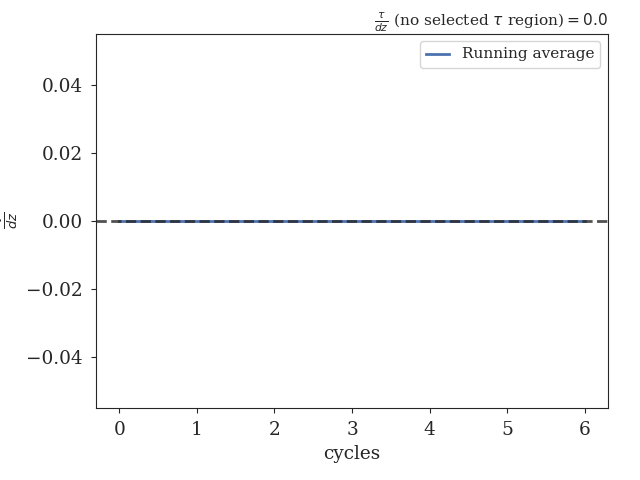
\includegraphics[width=0.33\linewidth]{taurun.png}
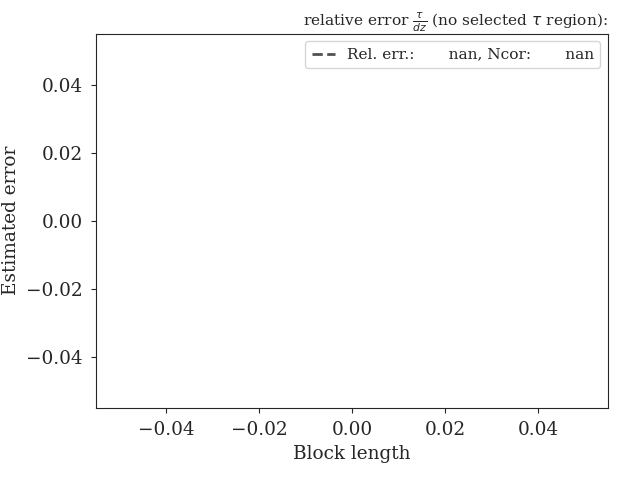
\includegraphics[width=0.33\linewidth]{tauerr.png}
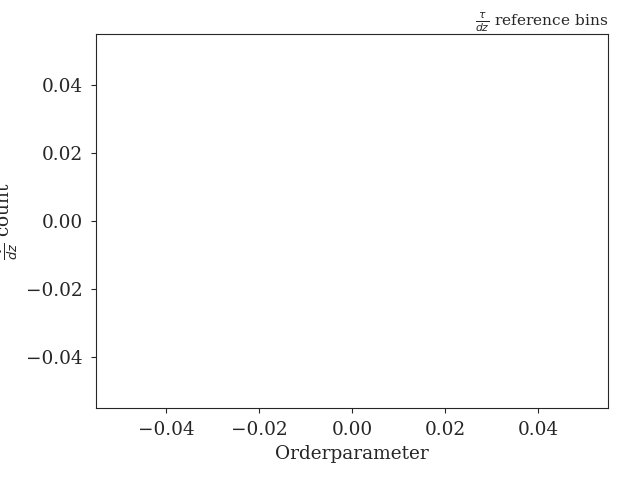
\includegraphics[width=0.33\linewidth]{tauref.png}
\clearpage


\end{center}


\section{Combined results}
\label{sec:combined}

The overall matched probability distributions are shown in the left figure
while the matched probability distribution is shown in the right figure below.
The overall crossing rate as a function of cycles
and its relative error block analysis are reported in the two following
plots, respectively.

\begin{center}
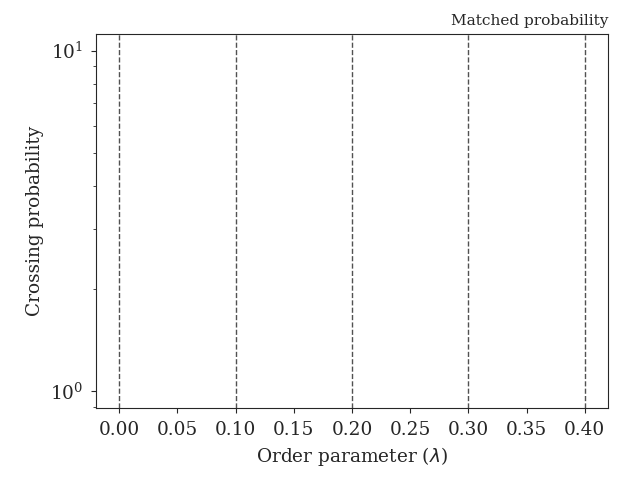
\includegraphics[width=0.45\linewidth]{matched-probability.png}%
\end{center}
\begin{center}
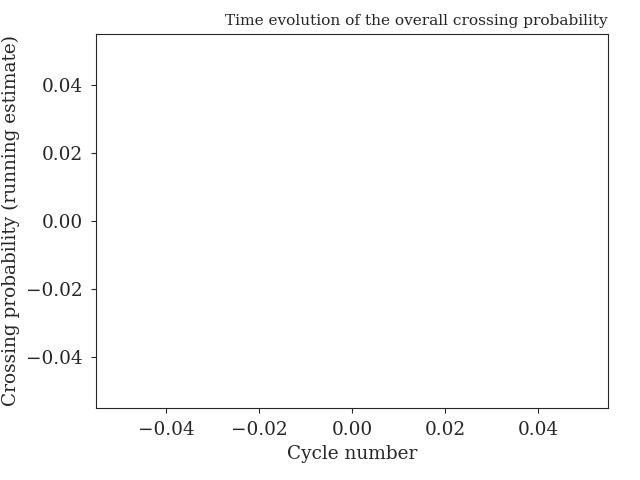
\includegraphics[width=0.45\linewidth]{overall-prun.png}%
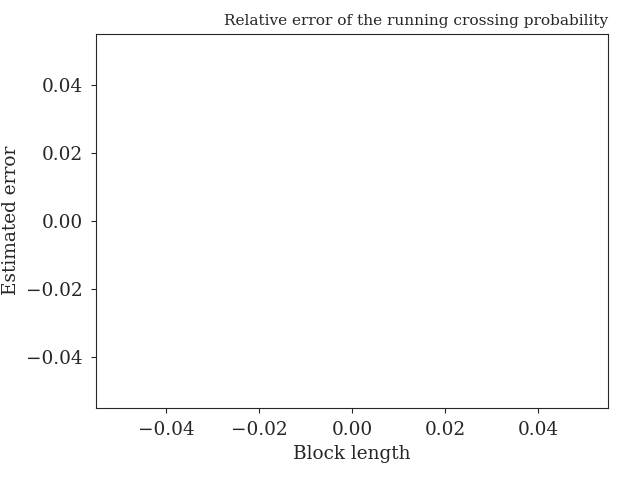
\includegraphics[width=0.45\linewidth]{overall-err.png}%
\end{center}

\clearpage

\section{Results for path ensembles}
The following interfaces were used in the simulation and in
the analysis:
\begin{longtable}{| c | c | c | c |}
\caption{Interfaces}\\
\hline
Ensemble & Left & Middle & Detect\\ \hline
$ [0^-]  $ & $-0.1000 $ & $ 0.0000 $ & $ 0.0000 $\\
$ [0^+]  $ & $ 0.0000 $ & $ 0.0000 $ & $ 0.1000 $\\
$ [1^+]  $ & $ 0.0000 $ & $ 0.1000 $ & $ 0.2000 $\\
$ [2^+]  $ & $ 0.1000 $ & $ 0.2000 $ & $ 0.3000 $\\
$ [3^+]  $ & $ 0.2000 $ & $ 0.3000 $ & $ 0.4000 $\\
\hline
\end{longtable}
\begin{longtable}{| c | c | c | c | c |}
\caption{Probabilities}\\
\hline
Ensemble & $\left\langle p^{ \pm}\right\rangle_{\text {full }}$ & $\left\langle p^{ \mp}\right\rangle_{\text {full }}$ & Error$^{ \pm}$ & Error$^{ \mp}$\\ \hline
$ [0^+]  $ & $ 0.000000 $ & $ 0.000000 $ & $ 0.000000 $ & $ 0.000000 $\\
$ [1^+]  $ & $ 0.000000 $ & $ 0.000000 $ & $ 0.000000 $ & $ 0.000000 $\\
$ [2^+]  $ & $ 1.000000 $ & $ 0.000000 $ & $ 0.000000 $ & $ 0.000000 $\\
$ [3^+]  $ & $ 0.666667 $ & $ 0.000000 $ & $ 0.333333 $ & $   nan    $\\
\hline
\end{longtable}
\begin{longtable}{| c | c | c | c | c |}
\caption{Pathensemble data}\\
\hline
Ensemble & TIS cycles & Shoot acc. ratio & Swap acc. ratio & Avg. path length\\ \hline
$ [0^-]  $ & $    7     $ & $ 0.500000 $ & $ 1.000000 $ & $ 3.285714 $\\
$ [0^+]  $ & $    9     $ & $ 0.400000 $ & $ 0.250000 $ & $10.000000 $\\
$ [1^+]  $ & $    6     $ & $ 0.750000 $ & $ 0.000000 $ & $123.833333$\\
$ [2^+]  $ & $    12    $ & $ 0.333333 $ & $ 0.500000 $ & $164.750000$\\
$ [3^+]  $ & $    4     $ & $ 1.000000 $ & $ 0.500000 $ & $559.250000$\\
\hline
\end{longtable}
\clearpage


\subsection{Crossing probabilities}

\begin{center}
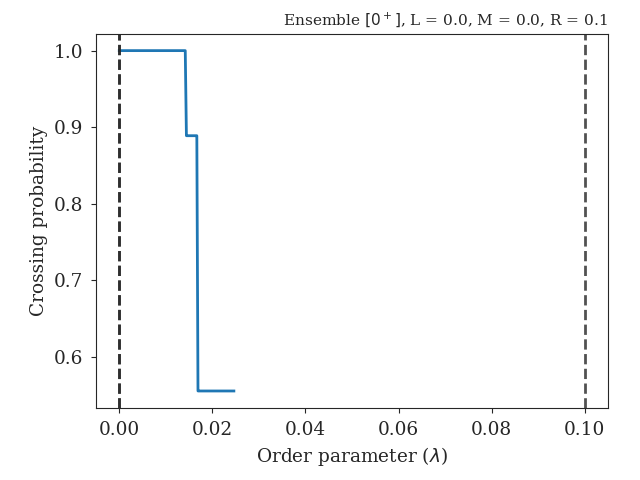
\includegraphics[width=0.33\linewidth]{001_pcross.png}%
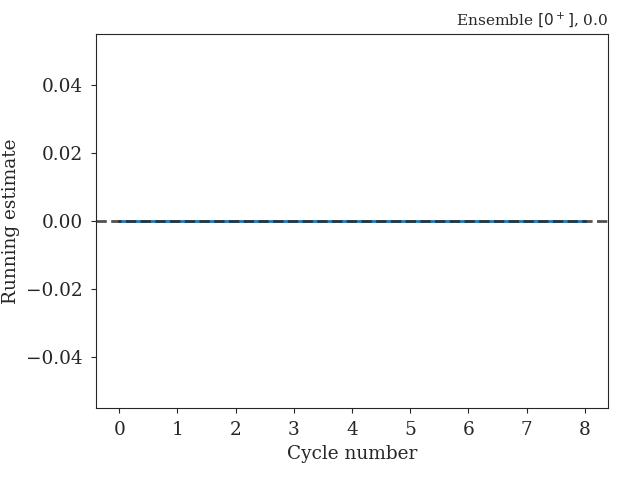
\includegraphics[width=0.33\linewidth]{001_prun_sl.png}%
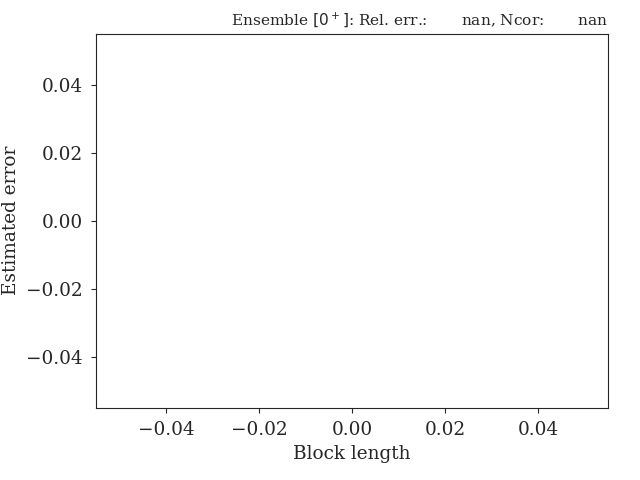
\includegraphics[width=0.33\linewidth]{001_perror_sl.png}%
\end{center}
\begin{center}
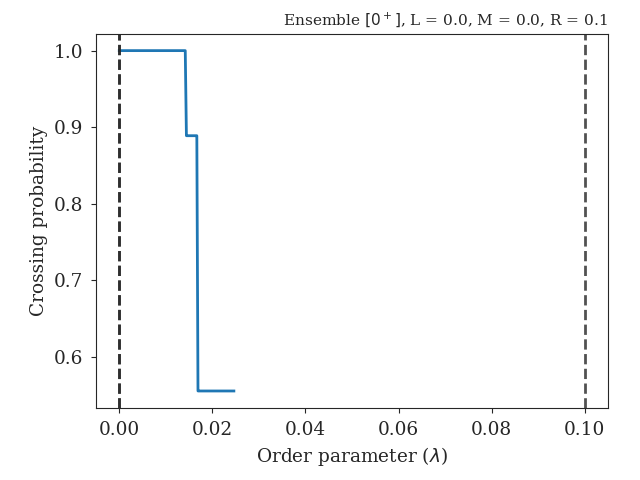
\includegraphics[width=0.33\linewidth]{001_pcross.png}%
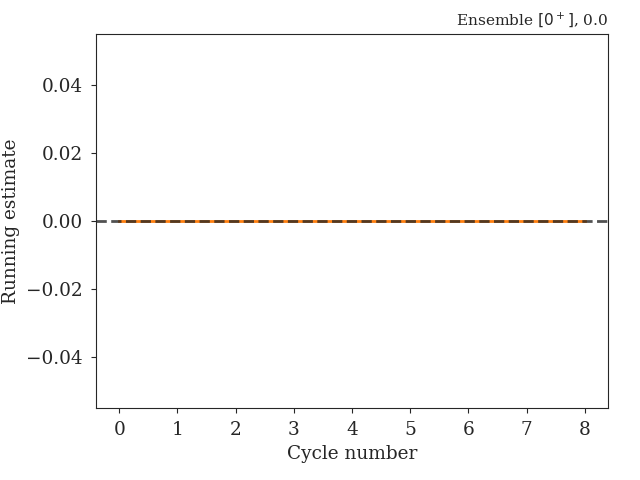
\includegraphics[width=0.33\linewidth]{001_prun_sr.png}%
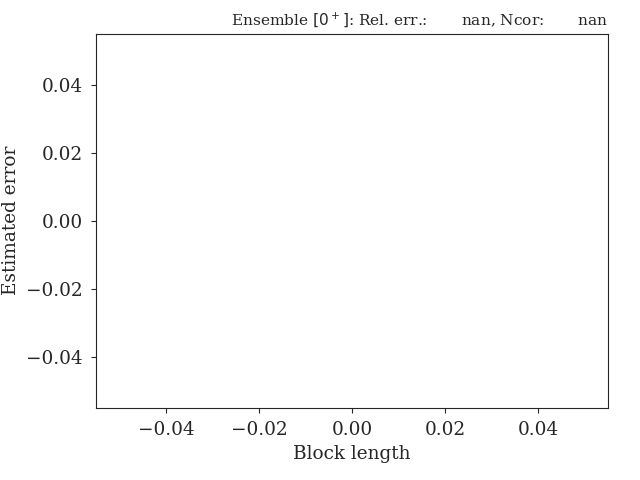
\includegraphics[width=0.33\linewidth]{001_perror_sr.png}%
\end{center}

\begin{center}
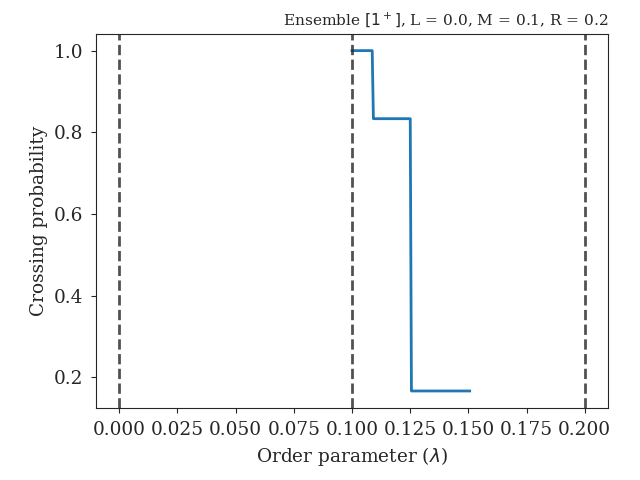
\includegraphics[width=0.33\linewidth]{002_pcross.png}%
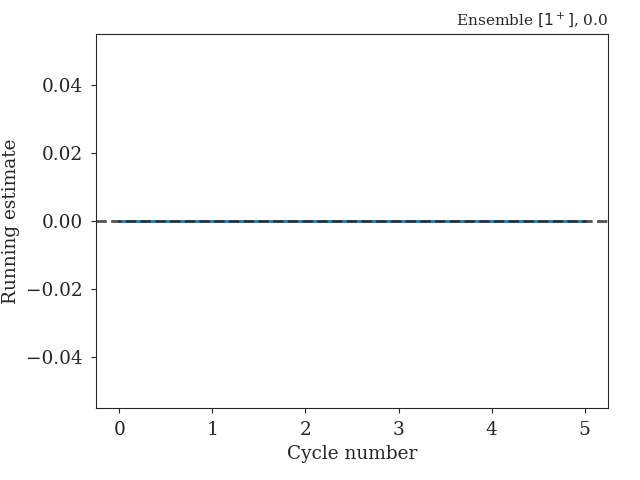
\includegraphics[width=0.33\linewidth]{002_prun_sl.png}%
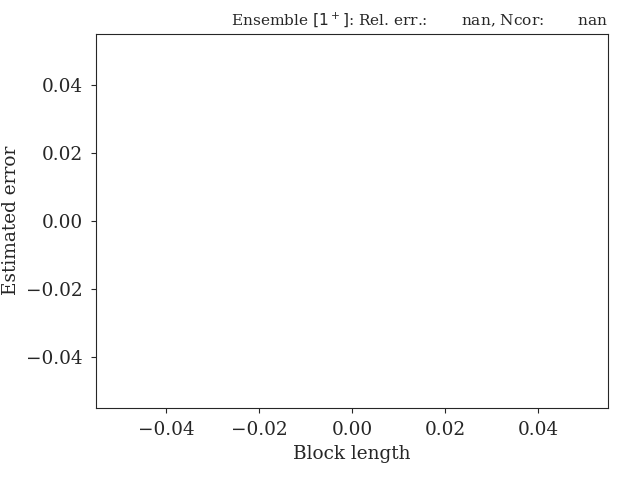
\includegraphics[width=0.33\linewidth]{002_perror_sl.png}%
\end{center}
\begin{center}
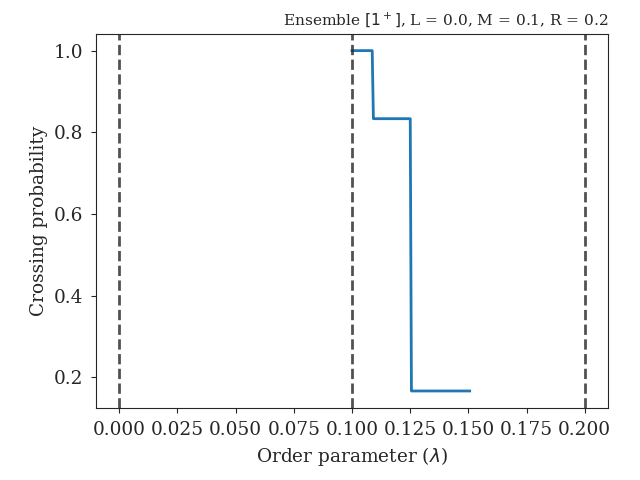
\includegraphics[width=0.33\linewidth]{002_pcross.png}%
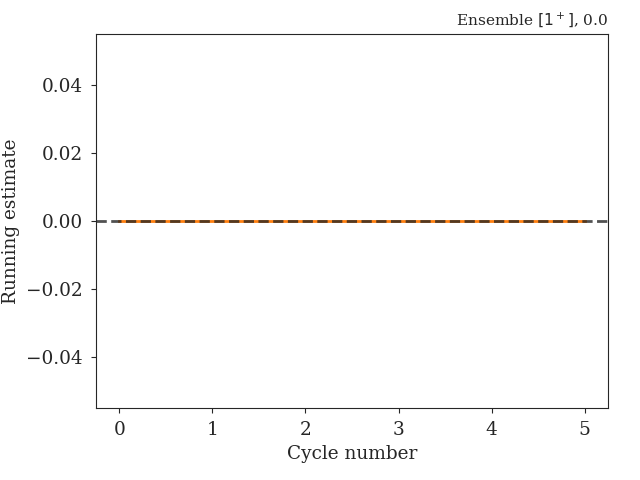
\includegraphics[width=0.33\linewidth]{002_prun_sr.png}%
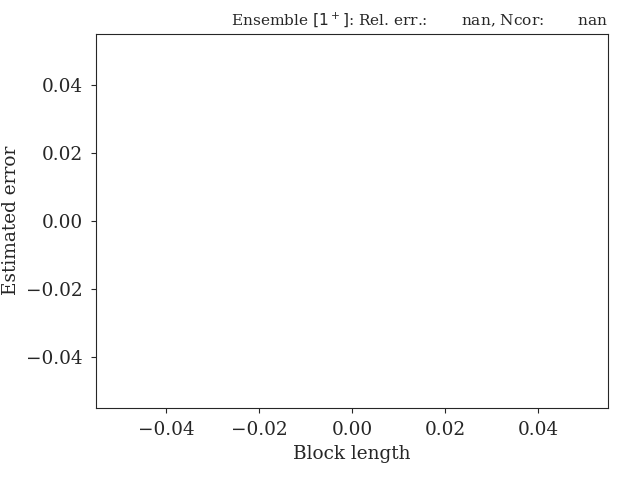
\includegraphics[width=0.33\linewidth]{002_perror_sr.png}%
\end{center}

\begin{center}
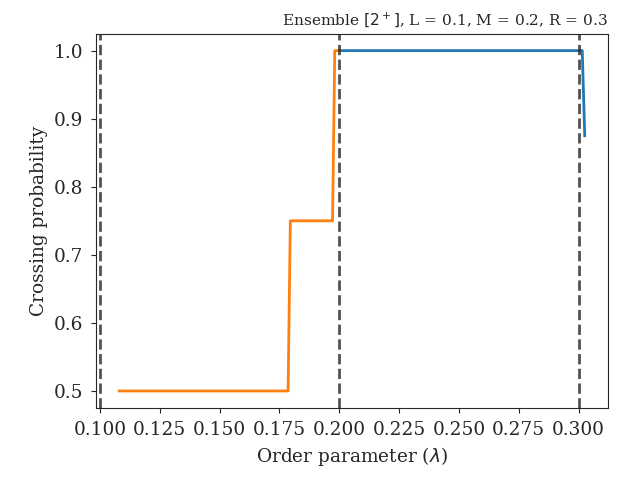
\includegraphics[width=0.33\linewidth]{003_pcross.png}%
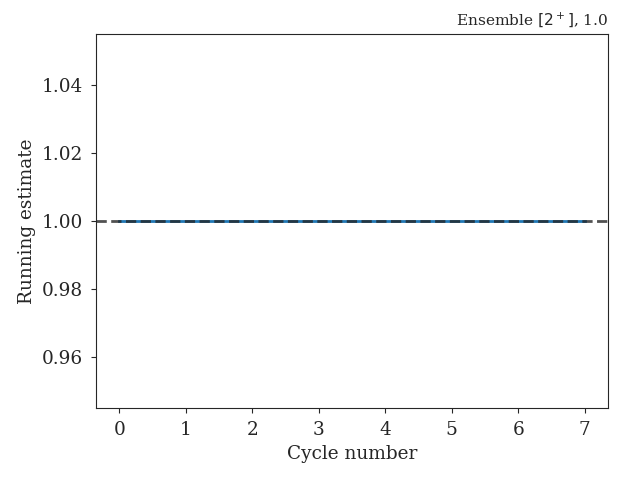
\includegraphics[width=0.33\linewidth]{003_prun_sl.png}%
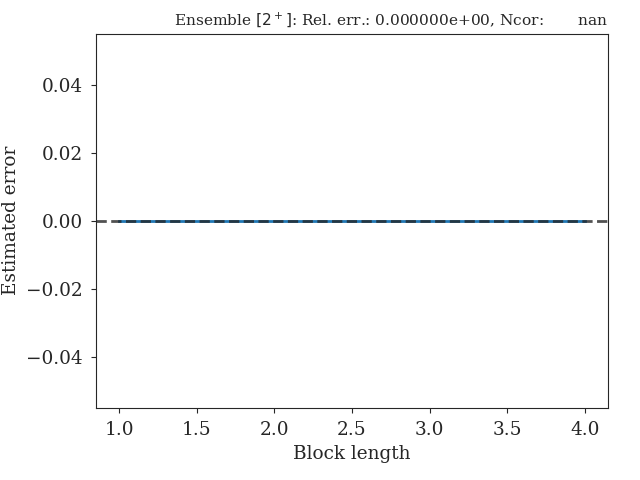
\includegraphics[width=0.33\linewidth]{003_perror_sl.png}%
\end{center}
\begin{center}
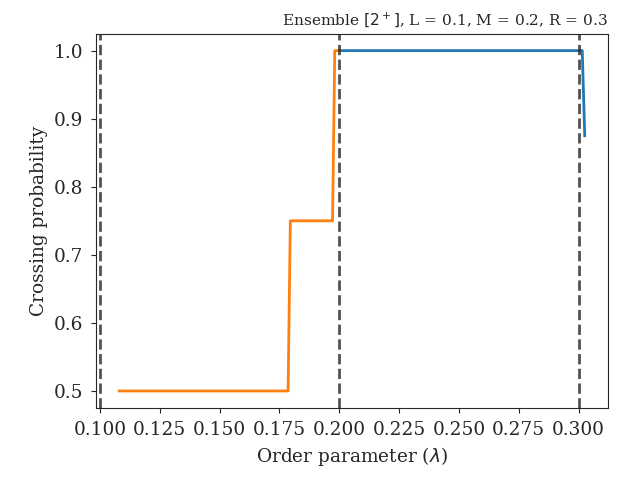
\includegraphics[width=0.33\linewidth]{003_pcross.png}%
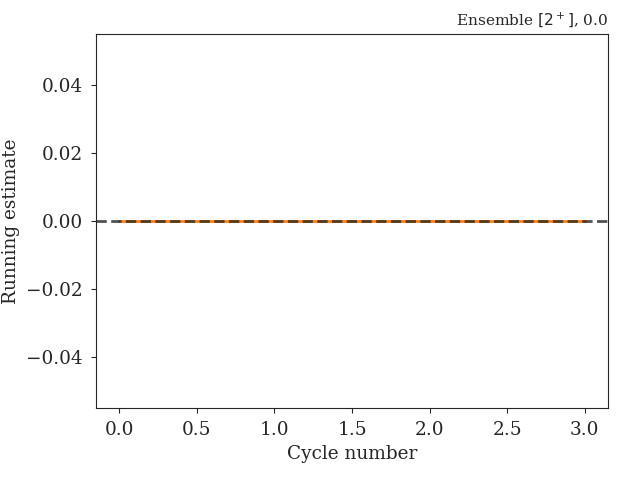
\includegraphics[width=0.33\linewidth]{003_prun_sr.png}%
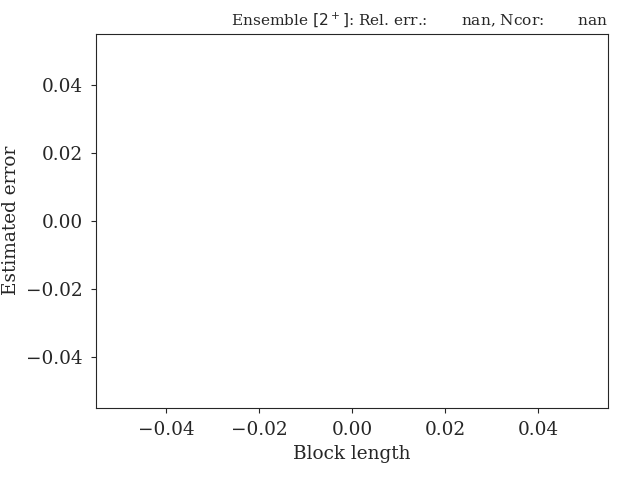
\includegraphics[width=0.33\linewidth]{003_perror_sr.png}%
\end{center}

\begin{center}
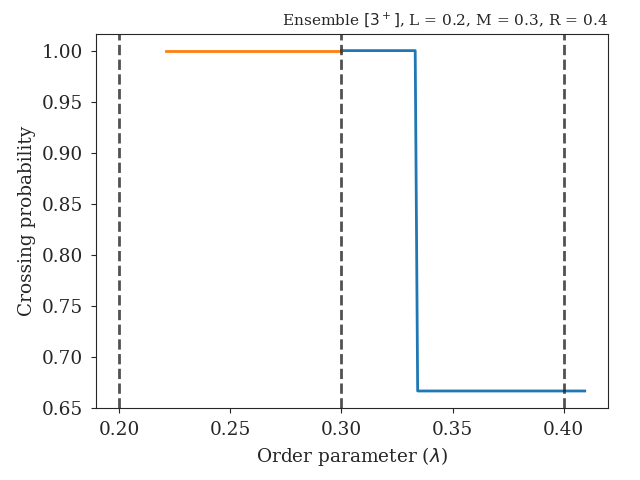
\includegraphics[width=0.33\linewidth]{004_pcross.png}%
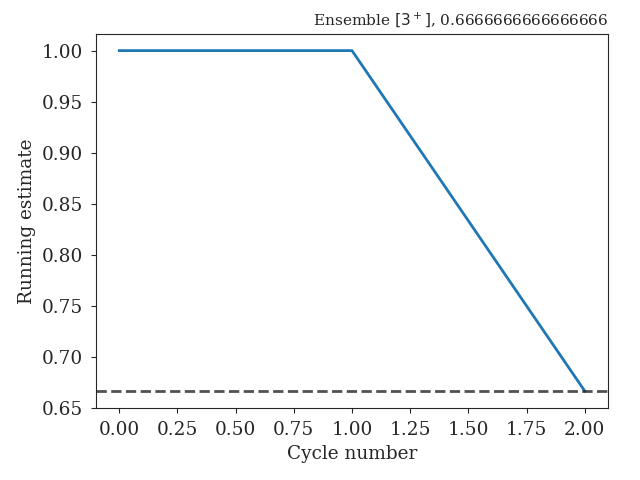
\includegraphics[width=0.33\linewidth]{004_prun_sl.png}%
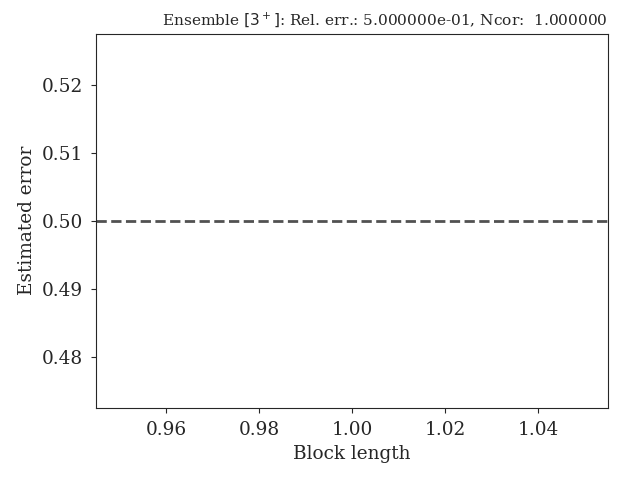
\includegraphics[width=0.33\linewidth]{004_perror_sl.png}%
\end{center}
\begin{center}
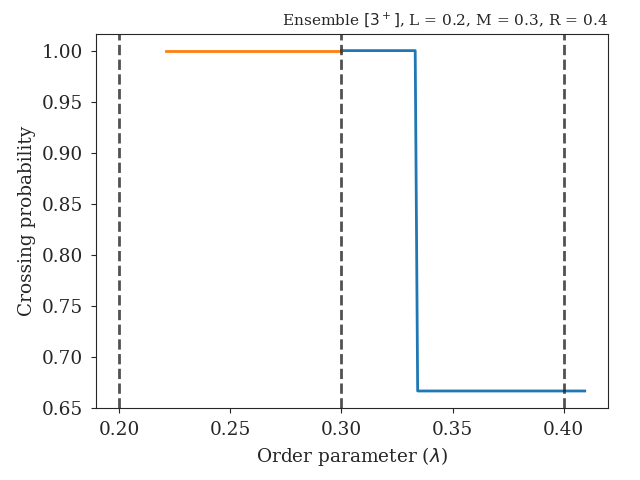
\includegraphics[width=0.33\linewidth]{004_pcross.png}%
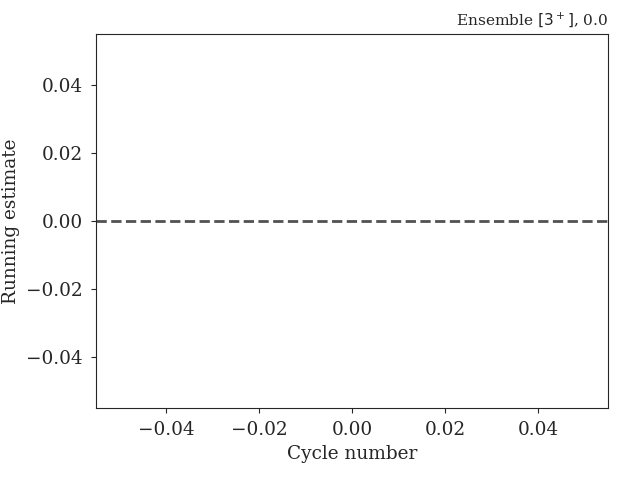
\includegraphics[width=0.33\linewidth]{004_prun_sr.png}%
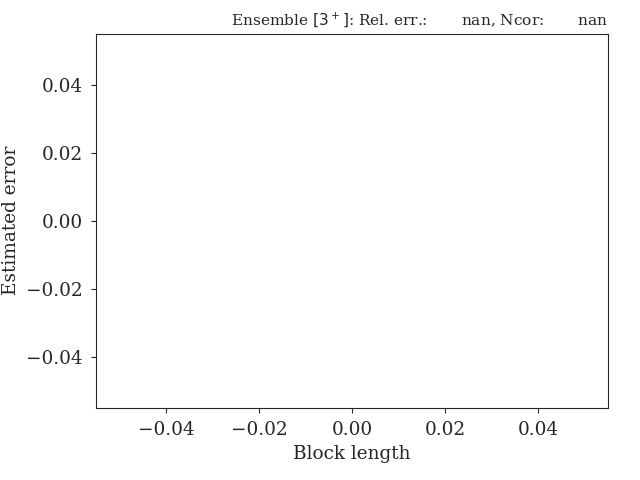
\includegraphics[width=0.33\linewidth]{004_perror_sr.png}%
\end{center}

\clearpage

\subsection{Distributions for path lengths and shooting moves}
The average path lengths in the different ensembles are given in
the table below and some distributions for the path lengths and
shooting moves can also be found here:

\begin{center}
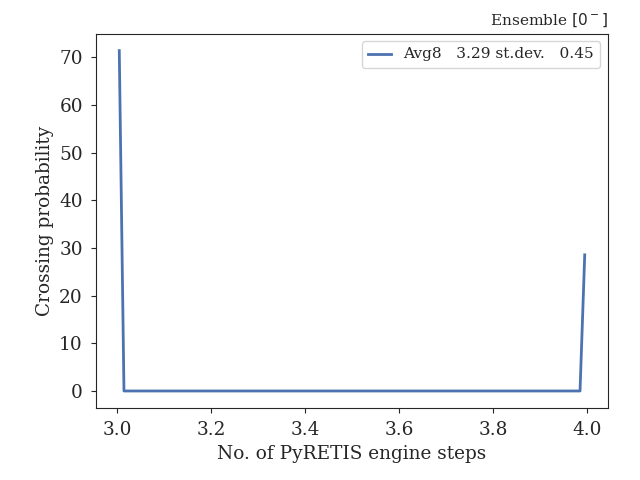
\includegraphics[width=0.45\linewidth]{000_lpath.png}%
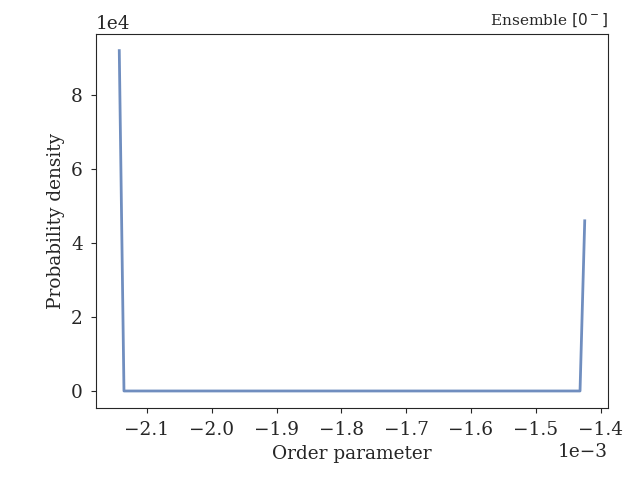
\includegraphics[width=0.45\linewidth]{000_shoots.png}%
\end{center}


\begin{center}
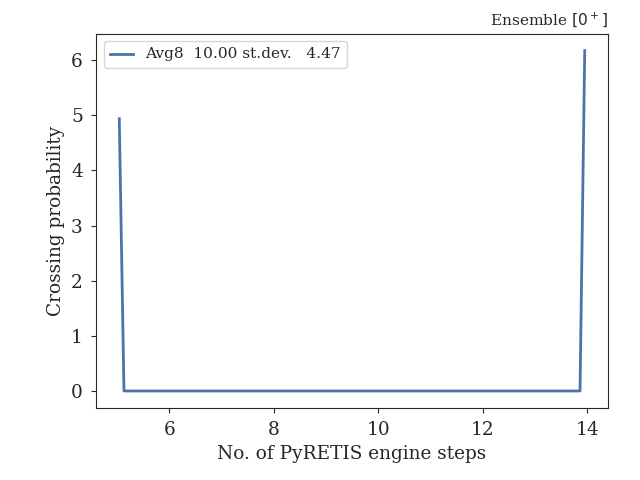
\includegraphics[width=0.45\linewidth]{001_lpath.png}%
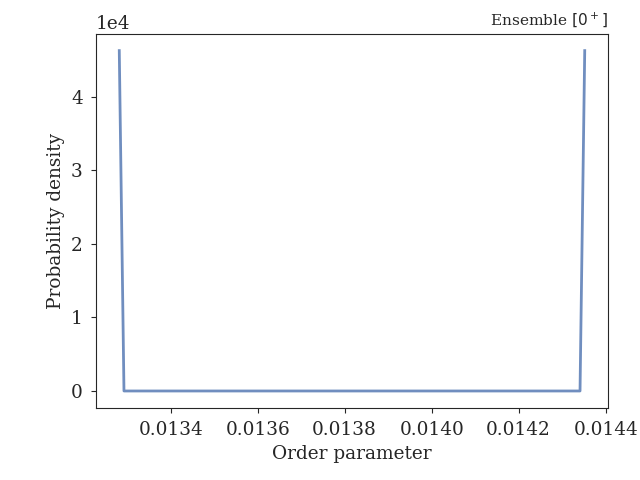
\includegraphics[width=0.45\linewidth]{001_shoots.png}%
\end{center}

\begin{center}
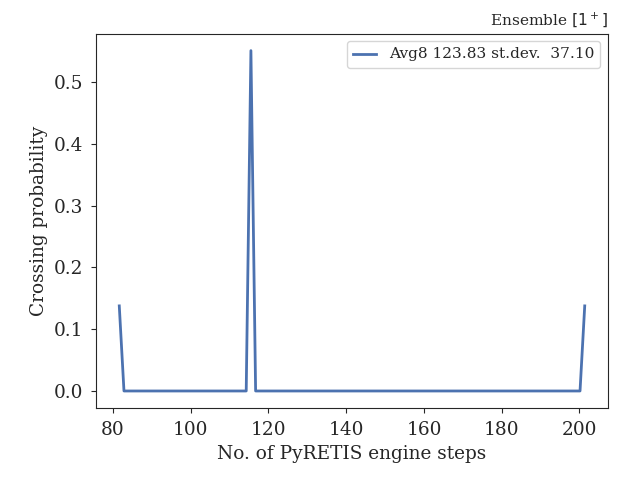
\includegraphics[width=0.45\linewidth]{002_lpath.png}%
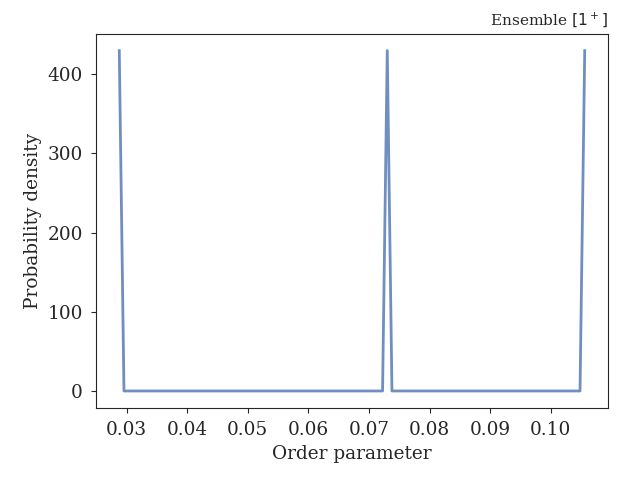
\includegraphics[width=0.45\linewidth]{002_shoots.png}%
\end{center}

\begin{center}
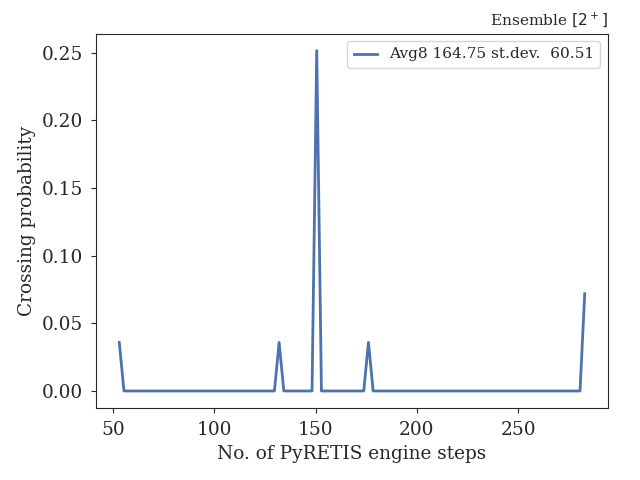
\includegraphics[width=0.45\linewidth]{003_lpath.png}%
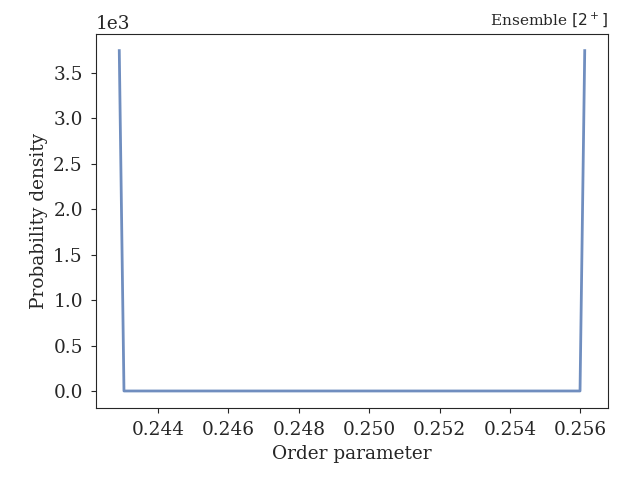
\includegraphics[width=0.45\linewidth]{003_shoots.png}%
\end{center}

\begin{center}
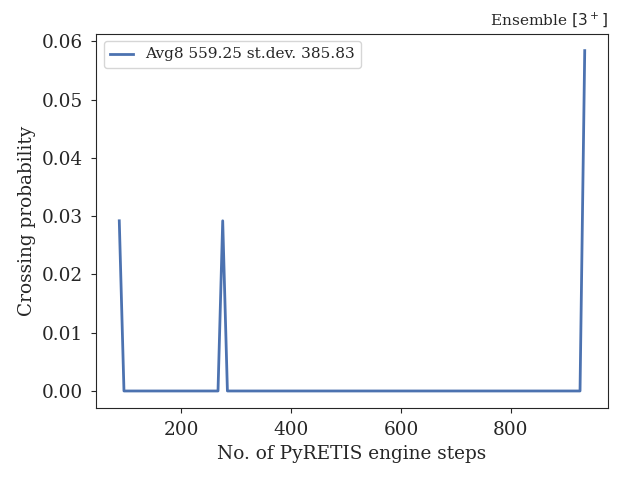
\includegraphics[width=0.45\linewidth]{004_lpath.png}%
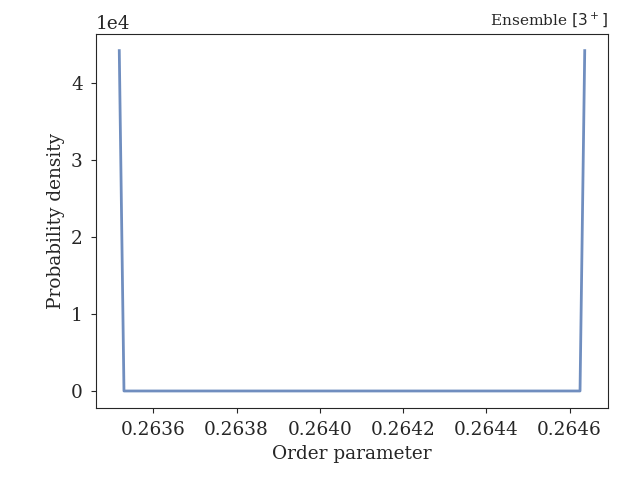
\includegraphics[width=0.45\linewidth]{004_shoots.png}%
\end{center}

\clearpage

\end{document}